\setAuthor{Oleg Košik}
\setRound{lõppvoor}
\setYear{2022}
\setNumber{G 7}
\setDifficulty{7}
\setTopic{TODO}

\prob{Veeuputus}
Tänava kanalisatsioon on ehitatud selliselt, et vihmasaju korral koguneb vihmavesi kõigepealt tänava all kulgevasse kraavi, kust omakorda juhitakse vesi ära sadeveetorustiku kaudu. Sadeveetorustiku ummistuse tõttu suudab see aga tagada sadevee äravoolu ainult 50\% võimsusel maksimaalsest võimalikust. Ükskord paduvihma ajal juba 6 minutit peale vihma algust sai kraav täis ning vesi tungis tänavale. Graafikul (pöördel) on toodud sademete koguhulga $h$ sõltuvus ajast $t$ alates paduvihma algusest. \\
Peale paduvihma lõppemist tehtud arvutused näitasid, et isegi juhul, kui sadeveetorustik poleks ummistunud, poleks see uputusest päästnud ning kraav oleks täitunud 9 minutit peale vihma algust.\\
Milline pidanuks olema töökorras torustiku äravoolu minimaalne võime (liitrit minutis $\SI{1} {m^2}$ pinna kohta), et uputust ei oleks tekkinud? 

\hint

\solu
\
Paneme tähele, et \SI{1}{l\per m^2}=\SI{1}{mm} ehk otsitav torustiku äravool on arvuliselt võrdne äraveetavate sademete hulgaga millimeetrites.

Olgu $h_6=\SI{22}{\mm}$ sademete koguhulk 6 minuti järel ning $h_9=\SI{28}{\mm}$ omakorda 9 minuti järel, $H$ mitu millimeetrit sademeid suudab endas mahutada kraav (kui äravoolu ei oleks) ning $u$ töökorras torustiku sademete äravoolu kiirus millimeetrites minutis.

Saame võrrandid
\[
h_6 = H +0.5 u \cdot \SI{6}{\min}
\]
ja
\[
h_9 = H + u \cdot \SI{9}{\min}
\]
Sellest võrrandisüsteemist leiame $H=\SI{19}{\mm}$.

Olgu otsitud äravoolu kiirus $u_x$. Siis sirge $h(t)=H+u_xt$ näitab, kui palju suudab kanalisatsioonisüsteem akumuleerida vett maksimaalselt igal ajahetkel ($H$ on kraavi panus $u_xt$ sadeveetorustiku panus). Selleks, et uputus ei tekiks, peab sademete koguhulga graafik jääma alati sellest sirgest allapoole. Kiirus $u_x$ on minimaalne siis, kui see sirge on graafiku puutuja. Tõmbame niisiis graafikult puutuja, mis läbib punkti $(0,H)$. Selle puutuja tõus on otsitav kiirus $u_x$. Mõõtmised annavad meile $u_x=\SI{1.23}{mm/min}=\SI{1.23}{\L\per\m\squared}$ minutis.

\begin{figure}[h]
	\vspace{-1em}
    \centering
    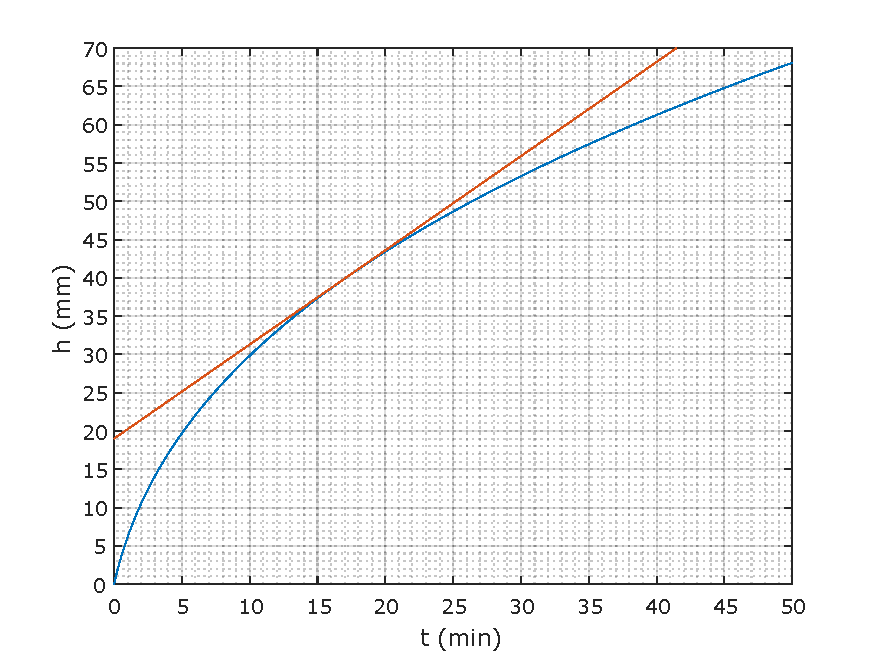
\includegraphics[width=0.75\linewidth]{2022-v3g-07-yl.pdf}
\end{figure}
\probend